%%%% ijcai19-multiauthor.tex

\typeout{IJCAI-19 Multiple authors example}

% These are the instructions for authors for IJCAI-19.

\documentclass{article}
\pdfpagewidth=8.5in
\pdfpageheight=11in
% The file ijcai19.sty is NOT the same than previous years'
\usepackage{ijcai19}

% Use the postscript times font!
\usepackage{times}
\usepackage{soul}
\usepackage[hyphens]{url}
\usepackage[hidelinks]{hyperref}
\usepackage[utf8]{inputenc}
\usepackage[small]{caption}
\usepackage{graphicx}
\usepackage{amsmath}
\usepackage{booktabs}
\urlstyle{same}

% the following package is optional:
%\usepackage{latexsym} 

\bibliographystyle{IEEEtran}


% Following comment is from ijcai97-submit.tex:
% The preparation of these files was supported by Schlumberger Palo Alto
% Research, AT\&T Bell Laboratories, and Morgan Kaufmann Publishers.
% Shirley Jowell, of Morgan Kaufmann Publishers, and Peter F.
% Patel-Schneider, of AT\&T Bell Laboratories collaborated on their
% preparation.

% These instructions can be modified and used in other conferences as long
% as credit to the authors and supporting agencies is retained, this notice
% is not changed, and further modification or reuse is not restricted.
% Neither Shirley Jowell nor Peter F. Patel-Schneider can be listed as
% contacts for providing assistance without their prior permission.

% To use for other conferences, change references to files and the
% conference appropriate and use other authors, contacts, publishers, and
% organizations.
% Also change the deadline and address for returning papers and the length and
% page charge instructions.
% Put where the files are available in the appropriate places.

\title{Application of Artificial Intelligent in Healthcare}

\author{
Ethan Garnier$^1$\footnote{Contact Author}\and
Matthew Tidd$^2$\And
Minh Nguyen$^{2}$
\affiliations
$^1$Electrical and Computer Engineering Department, UNB\\
$^2$Mechanical Engineering Department, UNB
\emails
\{ethan.garnier78, matthew.tidd, mnguyen6\}@unb.ca
}

\begin{document}

\maketitle

\begin{abstract}
This short example shows a contrived example on how to format the authors' information for {\it IJCAI--19 Proceedings} using \LaTeX{}.
\end{abstract}

\section{Introduction}

This short example shows a contrived example on how to format the authors' information for {\it IJCAI--19 Proceedings}.
\section{History of AI in Healthcare}
\subsection{Recent Developments in Healthcare AI}
Ever since the age of big data, there has been a surge in AI developments. 
This acceleration originates from several factors, including the wealth of data collected by big tech, the decreased cost of computational power, developments of more efficient machine learning techniques, and the availability of open-source machine learning packages
The healthcare and medical fields are no exclusion from this wave of AI developments. 
In fact, AI and ML application is an active field of research, receiving attention from researchers, medical stakeholders, and policy makers.
The immersion of the technology in the medical field is evident in the growth of FDA-approved AI/ML-enabled medical devices in \autoref{fig:FDA} \cite{FDA_artificial_nodate}

\begin{figure}[htbp]
    \centering{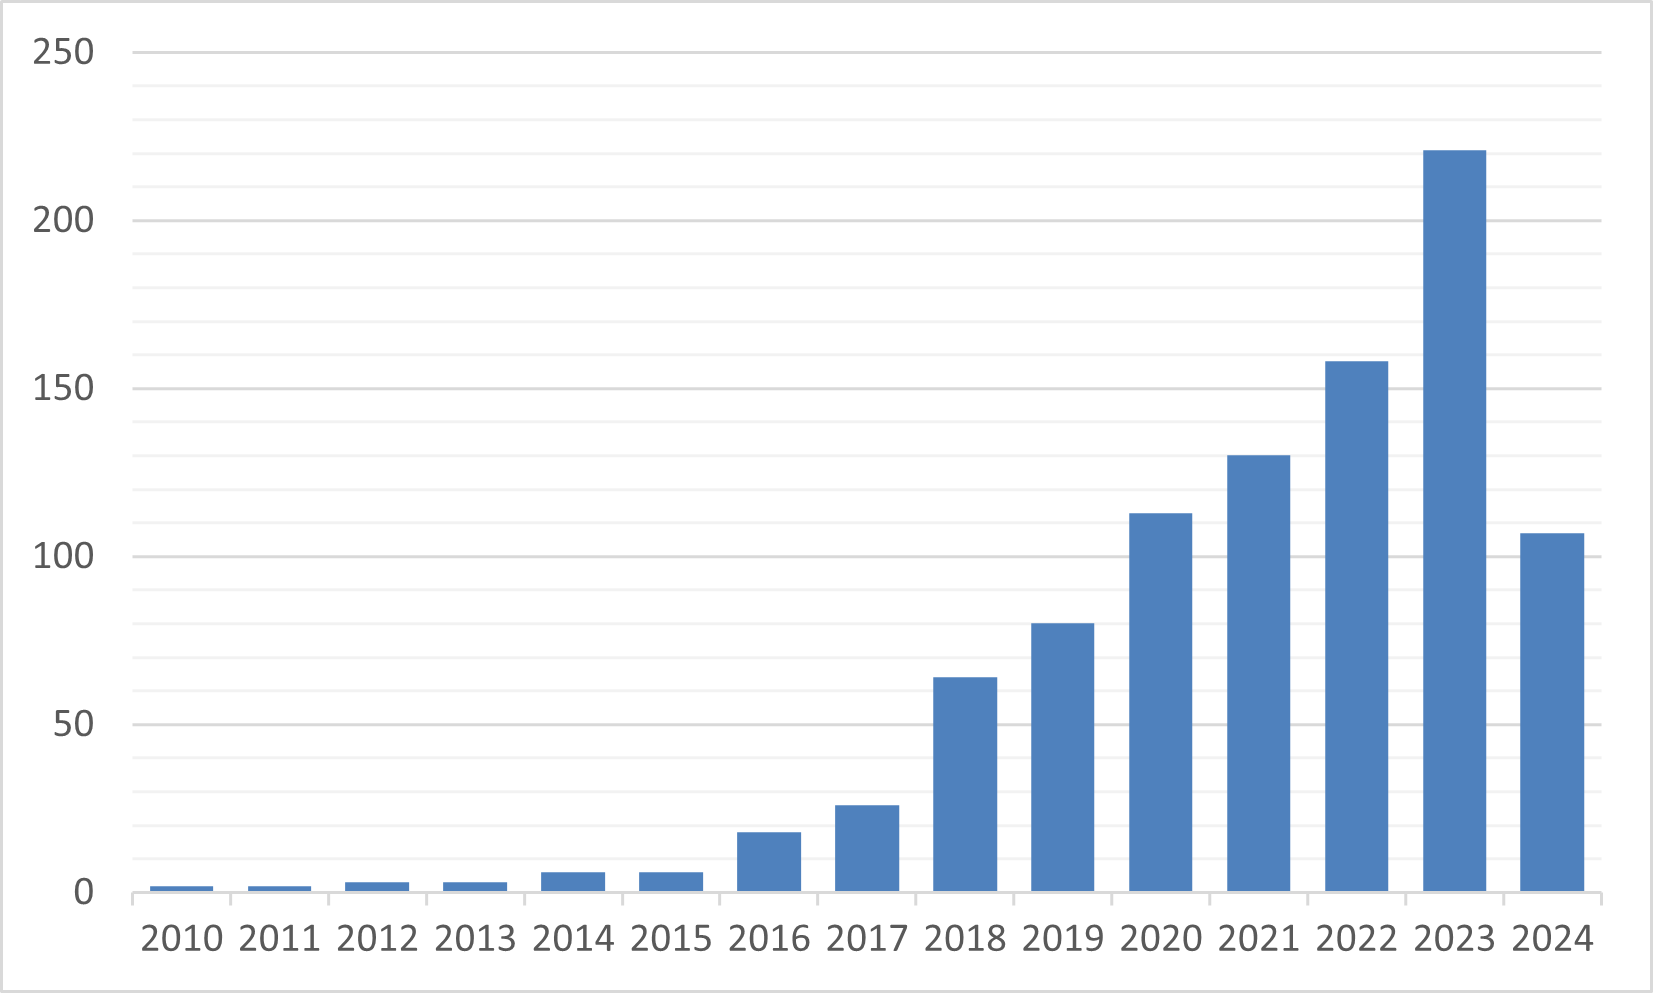
\includegraphics[scale=0.6]{Resources/Growth in ML enabled devices.png}}
    \caption{Number of FDA-approved AI/ML-enabled medical devices since 2010} 
    \label{fig:FDA}
\end{figure}

\subsubsection{Radiology}
In radiology, machine learning is a powerful tool that can help physisicians with CT scan and MRI scan to diagnose diseases and extract latent insights from the scans. Some example work include
\begin{itemize}
    \item Classification of triple negative breast canser using ultrasound images \cite{wu_machine_2019}
    \item Detection of pulmonary lung nodules from CT scans by convolutional neural network \cite{van_ginneken_off--shelf_2015}
    \item Pneumonia detection from chest X-rays using modern deep learning \cite{rajpurkar_chexnet_2017}
    \item Detection of breast mass from mammography scans using convolutional neural networks \cite{arevalo_convolutional_2015}
\end{itemize} 

\subsubsection{Dermatology}
In dermatology diagnosis, visual inspection is still the main method for determining the severity of a skin abnormalities or lesions. 
Machine learning emerges as an effective method for automating this process as they can learn the latent features that differentiate between benign and malignant lesions in skin melanoma. 
As early as 1994, the research in \cite{ercal_neural_1994} applied neural network to automate the classification of malignant melanoma from benign tumors that share similar characteristics as melanoma.
The author 
In \cite{esteva_dermatologist-level_2017}, a convolutional neural network was trained on 100,000 clinical images of skin cancer and achieved an accuracy similar to that of a dermatologist.
Once these models have been trained extensively on computationally efficient hardware, they can be packaged and deployed on mobile devices to make inferences on skin lesions. 
This can further increase the accessibility of machine learning functionalities to the wider population.



\subsubsection{Hematology}
In the case of hematological diseases, early prediction can help prevent progression and complication of blood disorders such as leukemia and lymphoma. 
Traditionally, practitioners diagnose hematological conditions by phenotypic assessment of peripheral blood nd bone marrow samples. 
However, diagnostic ambiguity often occurs in such manual process depending on the operator experience and capabilities. 
The reproducibility of clinical results also varies amongst skilled hematologists and pathologists \cite{walter_artificial_2023}.
Therefore, there is a desire for an automated process for reduced reliance on expert knowledge and increased consistency in data interpretation.
Given its predictive power, machine learning implementation in disease diagnosis from blood samples is an active research topic.

In 2014, early developments of automated systems leveraging machine learning had limited capabilities, performing tasks such as blood cell counting or classificiation of lymphoid cell types \cite{alomari_automatic_2014,alferez_automatic_2014,alferez_automatic_2015}.
In \cite{guncar_application_2018}, two ML models were developed to predict hematologic disease.
One of them was trained on all available blood test parameters and the other trained on a reduced set of parameters usually obtained from patient admittance.
When this input is paired with the knowledge of the five most likely diseases, the models achieve predictive performance on par with haematology specialists
The research in \cite{cheuque_efficient_2022} employed a two-stage CNN architecture to classifies four types of white blood cells (leukocytes).
The first layer of CNN leveraged a Faster R-CNN network to delineate the regions of interest and differentiate mononuclear cells from polymorphonuclear cells. 
The seconds layer consists of two parallels CNN with the MobileNet architectures and transfer learning to further categorize the subclasses of leukocytes. 
The lightweight architecture and parallelization allows for faster inferencing time.



\subsubsection{Ophthamology}
In the field of ophthamology, a fundoscopy is a non invasive procedure for inestigating the patient's fundus, or the back of their eyes, to diagnose vision conditions and risk factors leading to vision loss.
These detected factors can be used to predict the onset of diseases such as diabetic retinography, glaucoma, retina neoplasms, and macular degeneration \cite{kumar_artificial_2023}

Diabetic retinography (DR) is a condition where high blood sugar level causes damaged vessel in the retina. 
This condition is one of the common causes of vision loss and impairment amongst American living with diabetes and working age adults \cite{commissioner_fda_2020,abramoff_pivotal_2018}.
In 2018, the FDA approved of IDx-DR, the first AI-enabled system for detecting DR.
The research in \cite{abramoff_improved_2016} and \cite{abramoff_pivotal_2018} leveraged a multilayer CNN to train independent detectors for the anatomy and the characteristics of DR, including microaneurysms, hemorhages, and lipoprotein exudates.
The results of these detectors are combined to return the levels of the diseases. 
The study in \cite{sayres_using_2019} implemented an Inception V4 model, also a CNN architecture, to detect the severity grade of DR and provide a heatmap of regions of interest 



\subsubsection{Oncology}
The integration of AI and ML systems in cancer treatment is an active branch of research.
A potential use of AI in this field of research is radiotherapy dosage optimization and image segmentation for tissue abnormality detection, where the algorithms have shown promising improvements compared to manual planning.



\section{Challenges}
\subsection{Trust}
\subsection{Accountability}
\subsection{Data privacy and protection}
AI technologies depend on a vast amount of patient data and record to make accurate predictions when subjected to unseen data.
However, in the event of a database violation or data breach, confidential patient information can be exploited for malicious intentions (identity theft, social stigma, discrimination,...).
This can put a mental burden on the patient suceptible to the violation and other relevant stakeholders.
Therefore, adequate law and guidelines are crucial to regulate the application of AI in medical and prevent misuse of data


The data gathering and handling of health data in the US is controversial, raising legal and ethical privacy questions \cite{price_privacy_2019}.
Although the data can originate from various sources, such as healthcare providers, insurance claim, and wearable devices, US privacy law operates in different extents depending on the data source.
This law also depends on the custodian of the data. Under the Health Insurance Portability and Accountability Act (HIPAA), the federal Privacy Rule only governs data handling between the conventional entities, such as healthcare providers, health insurance provides, patients, and intermediaries. 
However, \cite{price_privacy_2019} pointed out existing gap in HIPAA regulation.
Although, HIPAA protect patient privacy from health data breach via a deindentifying process, patient data can be reidentified through data triangulation from other datasets.


Furthermore, a more fundamental problem is the amount of health related data not regulated under HIPAA \cite{price_privacy_2019}. 
Originally enacted to regulate data privacy in health records and between covered entities, HIPAA does not account for health data generate outside the confinement of these covered entities. 
In the big data world, tech companies are displacing covered entities in the collection of health information and personal data from online searches, application logs, and smart wearable devices.

\section{Conclusion}

\section{Template notes}

\subsection{Author names}

Each author name must be followed by:
\begin{itemize}
    \item A newline {\tt \textbackslash{}\textbackslash{}} command for the last author.
    \item An {\tt \textbackslash{}And} command for the second to last author.
    \item An {\tt \textbackslash{}and} command for the other authors.
\end{itemize}

\subsection{Affiliations}

After all authors, start the affiliations section by using the {\tt \textbackslash{}affiliations} command.
Each affiliation must be terminated by a newline {\tt \textbackslash{}\textbackslash{}} command. Make sure that you include the newline on the last affiliation too.

\subsection{Mapping authors to affiliations}

If some scenarios, the affiliation of each author is clear without any further indication (\emph{e.g.}, all authors share the same affiliation, all authors have a single and different affiliation). In these situations you don't need to do anything special.

In more complex scenarios you will have to clearly indicate the affiliation(s) for each author. This is done by using numeric math superscripts {\tt \$\{\^{}$i,j, \ldots$\}\$}. You must use numbers, not symbols, because those are reserved for footnotes in this section (should you need them). Check the authors definition in this example for reference.

\subsection{Emails}

This section is optional, and can be omitted entirely if you prefer. If you want to include e-mails, you should either include all authors' e-mails or just the contact author(s)' ones.

Start the e-mails section with the {\tt \textbackslash{}emails} command. After that, write all emails you want to include separated by a comma and a space, following the same order used for the authors (\emph{i.e.}, the first e-mail should correspond to the first author, the second e-mail to the second author and so on).

You may ``contract" consecutive e-mails on the same domain as shown in this example (write the users' part within curly brackets, followed by the domain name). Only e-mails of the exact same domain may be contracted. For instance, contracting ``person@example.com" and ``other@test.example.com" is not allowed because the domains are different.


% Bibliography/Reference Stuff
\bibliography{main}
\end{document}